\chapter{2023/9/20}\label{20230920}

\section{Vibration of string 弦的振动}\label{vibration-of-string-ux5f26ux7684ux632fux52a8}

We assume that the string below has tension (张力) \(T\) which is equal at every point on the string; the string is long enough so that \(\theta \ll 1\) and \(\xi \ll 1\).

\begin{center}
    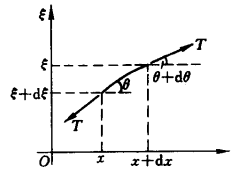
\includegraphics[height=90pt]{../assets/Vibration_of_String.png}
    \captionof{figure}{Demo of a string}
\end{center}

Consider the part of string in the picture Fig 4.1.

From Newton's Second Law of Motion (牛顿第二定律), we know that \[(\lambda \mathrm dx) {\partial^2 \xi \over \partial t^2 } = T \sin(\theta + \mathrm d\theta) - T \sin \theta.\]

Because \(\theta \ll 1\), we can approximate \(\sin \theta\) to \(\tan \theta\), and we can get: \begin{align*}
    (\lambda \mathrm dx) {\partial^2 \xi \over \partial t^2 } & = T \tan(\theta + \mathrm d\theta) - T \tan \theta \\
    & = T \left( \left. {\partial \xi \over \partial x} \right\vert _{x+\mathrm dx} - \left. {\partial \xi \over \partial x} \right \vert _x \right)\\
    & = T {\partial^2 \xi \over \partial x^2 } \mathrm dx,
\end{align*} and that brings us to \[\lambda {\partial^2 \xi \over \partial t^2 } = T {\partial^2 \xi \over \partial x^2 },\] \[{\lambda \over T} {\partial^2 \xi \over \partial t^2 } - {\partial^2 \xi \over \partial x^2 } = 0.\]

The velocity of the wave is \[c = \sqrt{T \over \lambda},\] and we can get \[{1 \over c^2} {\partial^2 \xi \over \partial t^2 } - {\partial^2 \xi \over \partial x^2 } = 0.\]

The equation above is on one dimension \(x\) only, and we can expand it to multiple dimensions \[{1 \over c^2} {\partial^2 \xi \over \partial t^2 } - \nabla ^2 \xi = 0,\] which is \[\left ( {1 \over c^2} {\partial^2 \over \partial t^2 } - \nabla ^2 \right ) \xi = \Box \xi = 0.\]

\section{Zero-Point Energy 零点能}\label{zero-point-energy-ux96f6ux70b9ux80fd}

\subsection*{(1) Simple Harmonic Oscillator 简谐振子}\label{simple-harmonic-oscillator-ux7b80ux8c10ux632fux5b50-1}

In classical mechanics we can have an SHO system, whose function can be written in the following ways:

\paragraph{Newtonian Mechanics 牛顿力学}\label{newtonian-mechanics-ux725bux987fux529bux5b66}

\[m \ddot x = -kx\] \[\ddot x + {k \over m } x =0 \] \[\ddot x + \omega^2 x =0, \ \omega=\sqrt{k \over m }.\]

\paragraph{Theoretical Mechanics 理论力学}\label{theoretical-mechanics-ux7406ux8bbaux529bux5b66}

\[L=T-V = {1 \over 2}m \dot x^2-{1 \over 2}k x^2\] \[{\partial L \over \partial \dot x} = m \dot x\] \[{\partial L \over \partial x} = -kx\]

From \[{\mathrm d \over \mathrm dt} {\partial L \over \partial \dot x}- {\partial L \over \partial x}=0,\] we know that \[{\mathrm d(m \dot x) \over \mathrm dt} - (-kx)=0, \] which is \[m \ddot x +kx = 0.\] \[\ddot x + \omega^2 x =0, \ \omega=\sqrt{k \over m }.\]

\subsection*{(2) Calculation of the zero-point energy 计算零点能}\label{calculation-of-the-zero-point-energy-ux8ba1ux7b97ux96f6ux70b9ux80fd}

Zero-point energy (ZPE) is the lowest possible energy that a quantum mechanical system may have.

Put the SHO system under quantum state (it becomes a \textbf{quantum harmonic oscillator} 量子谐振子), and we can get a minimum energy for it.

To calculate this ``minimum energy'', we start from Heisenberg Uncertainty Principle: \[\Delta x \cdot \Delta p \geq {\hbar \over 2}.\]

For the \textbf{lowest possible} energy, we need to have \[\Delta x \cdot \Delta p = {\hbar \over 2},\] which means \[\Delta p = {\hbar \over 2 \Delta x }.\]

From energy \[E = \dfrac{p^2}{2m}+ U = \dfrac{p^2}{2m} + {1 \over 2} m \omega^2 x^2,\] we can see that \begin{align*}
    \Delta E & = \dfrac{(\Delta p)^2}{2m} + {1 \over 2} m \omega^2 (\Delta x)^2 \\
    & = {{\left(\dfrac{\hbar}{ 2 \Delta x }\right)}^2 \over 2m} + {1 \over 2} m \omega^2 (\Delta x)^2 \\
    & = {\hbar^2 \over 8m(\Delta x)^2} + {1 \over 2} m \omega^2 (\Delta x)^2 \\
    & \geq 2 \sqrt{{\hbar^2 \over 8m(\Delta x)^2} \cdot {1 \over 2} m \omega^2 (\Delta x)^2} \\
    & = {\hbar \omega \over 2},
\end{align*} where \(=\) holds \textbf{if and only if} \[{\hbar^2 \over 8m(\Delta x)^2} = {1 \over 2} m \omega^2 (\Delta x)^2,\] that is, \[\Delta x = \sqrt{\hbar \over 2 m \omega}.\]

\emph{有些学着很聪明,以为什么都懂,但是其实他只懂了30\%。}
\emph{有些学者看起来呆头呆脑,但是呆头呆脑的人做研究做得踏实,这才是我们真正需要的大聪明。}

\section{Stationary Schrödinger Equation 定态薛定谔方程}\label{stationary-schruxf6dinger-equation-ux5b9aux6001ux859bux5b9aux8c14ux65b9ux7a0b}

We have the wave function \(\Psi(x, t)\).

We can perform \textbf{separation of variables (分离变量)} to the function and have \[\Psi(x, t) = \Phi(x) \cdot \mathcal{T}(t).\]

From \[-{ \hbar^2 \over 2m }{\partial^2 \Psi(x, t) \over \partial x ^2 } + U \Psi(x, t) =\mathrm i\hbar {\partial \Psi(x, t) \over \partial t},\] we can get \[-{ \hbar^2 \over 2m } \mathcal{T}(t){\mathrm d^2 \Phi(x) \over \mathrm d x ^2 } + U \Phi(x) \mathcal{T}(t) =\mathrm i\hbar \Phi(x) {\mathrm d \mathcal{T}(t) \over \mathrm d t}.\]

Put \(\Phi\) and \(x\) on one side and \(\mathcal{T}\) and \(t\) on the other, and we can get \[\dfrac{-\dfrac{ \hbar^2 }{2m}\dfrac{\mathrm d^2 \Phi(x)}{\mathrm d x ^2 } + U \Phi(x) }{\Phi(x)} = \dfrac{\mathrm i\hbar \dfrac{\mathrm d \mathcal{T}(t) }{\mathrm d t}}{\mathcal{T}(t)}.\]

Because \textbf{all \(\Phi\) and \(x\) are on the left side and all \(\mathcal{T}\) and \(t\) are on the right}, this equation can only hold \textbf{if this equation is equal to a constant}, that is, \[\dfrac{-\dfrac{ \hbar^2 }{2m}\dfrac{\mathrm d^2 \Phi(x)}{\mathrm d x ^2 } + U \Phi(x) }{\Phi(x)} = \dfrac{\mathrm i\hbar \dfrac{\mathrm d \mathcal{T}(t) }{\mathrm d t}}{\mathcal{T}(t)}=\mathrm{const}.\]

Perform dimensional analysis (量纲分析) on the equation above and we can see that the dimension of the constant is energy (\(\mathrm{M^1L^2T^{-2}}\)).

Let this constant be \(E\), and \(E\) is called the \textbf{eigenenergy} (能量的本征值).

Let's look at the two parts separately:

\subsection*{(1)\({\mathcal{T}(t)}\)}\label{mathcaltt}

The right part is equal to \(E\), which means that \begin{align*}
    \dfrac{\mathrm i\hbar \dfrac{\mathrm d \mathcal{T}(t) }{\mathrm d t}}{\mathcal{T}(t)} & =E \\
    \dfrac{\mathrm d \mathcal{T}(t) }{\mathcal{T}(t)} & = -{\mathrm iE \over \hbar}\mathrm dt \\
    \int {\dfrac{\mathrm d \mathcal{T}(t) }{\mathcal{T}(t)}} & = -{\mathrm iE \over \hbar} \int {\mathrm dt} \\
    \ln \mathcal{T}(t) & = -{\mathrm iE \over \hbar} t +C \\
    \mathrm e^{\ln \mathcal{T}(t)} & = \mathrm e^{- \mathrm iEt / \hbar +C} \\
    \mathcal{T}(t) & = \mathcal{T}_0 \cdot \mathrm e^{- \mathrm iEt / \hbar},
\end{align*} where \(C\) is the constant of integration (积分常数), and \(\mathrm e^C = \mathcal{T}_0\).

\subsection*{(2)\(\Phi(x)\)}\label{phix}

We can easily get this equation which does not include time \(t\) in it: \[-\dfrac{ \hbar^2 }{2m}\dfrac{\mathrm d^2 \Phi(x)}{\mathrm d x ^2 } + U \Phi(x) =E\Phi(x),\] which is called \textbf{Stationary Schrödinger Equation (定态薛定谔方程)}.

Under the SHO case, \(U=\dfrac{1}{2}m\omega^2x^2\), and we have \[-\dfrac{ \hbar^2 }{2m}\dfrac{\mathrm d^2 \Phi(x)}{\mathrm d x ^2 } + \dfrac{1}{2}m\omega^2x^2 \Phi(x) =E\Phi(x).\] Its general solution is \[\Phi^*(x) = C \exp(-{\alpha \over 2} x^2).\]

Find the first and second order derivatives for \(\Phi^*\):

\[{\mathrm d\Phi^*(x) \over \mathrm dx} = -\alpha x\cdot C \exp(-{\alpha \over 2} x^2) = -\alpha x \cdot \Phi^*(x)\]

\[{\mathrm d^2\Phi^*(x) \over \mathrm dx^2} = -\alpha (1-\alpha x^2) \cdot C \exp(-{\alpha \over 2} x^2) = -\alpha (1-\alpha x^2) \cdot \Phi^*(x)\]

And we have \[-\dfrac{ \hbar^2 }{2m}(-\alpha)(1-\alpha x^2)\cdot \Phi^*(x)+\dfrac{1}{2}m\omega^2x^2 \Phi^*(x)=E \Phi^*(x)\]

\[-\dfrac{ \hbar^2 }{2m}(-\alpha)(1-\alpha x^2)+\dfrac{1}{2}m\omega^2x^2 =E \]

\[\dfrac{\alpha \hbar^2 }{2m}(1-\alpha x^2) = E\left(1 - \dfrac{m\omega^2}{2E}x^2\right).\]

Compare the two forms and we know that \[\left \{
\begin {array}{l}
    \dfrac{\alpha \hbar^2 }{2m} = E, \\[1.5ex]
    \alpha = \dfrac{m\omega^2}{2E},
    \end {array}
    \right.\] and we get \[\left \{
    \begin {array}{l}
    E = \dfrac{\omega \hbar}{2}, \\[1.5ex]
    \alpha = \dfrac{m\omega}{\hbar}.
\end {array}
\right.\]
